\documentclass{l4proj}

\usepackage{url}
\usepackage{fancyvrb}
\usepackage{caption}
\usepackage{placeins}

\usepackage[final]{pdfpages}


\begin{document}
\title{Algorithm Animator}
\author{Andrei-Mihai Nicolae}
\maketitle

\begin{abstract}
Understanding algorithms is both very common and hard for developers in general,
regardless of their level of expertise. Even the fundamental ones, such as Dijkstra's algorithm
for finding the shortest path between two nodes in a graph, are quite complicated to grasp. Many 
studies show that visualizing an algorithm and its steps make understanding it much easier. In
this report, we will present an Algorithm Animator built specifically for solving this problem 
in a modern, responsive and efficient manner. Among others, we will also show why certain design decisions (e.g. making it a native
desktop app instead of a basic jar, using material design for the user interface), the implementation choices and the
evaluation results make this tool a viable option for software engineers when it comes to learning different kinds of 
algorithms.
\end{abstract}

\educationalconsent

\tableofcontents
%==============================================================================
\chapter{Introduction}
\label{intro}
\pagenumbering{arabic}

Firstly, the starting point should be defining what an algorithm is.

\begin{figure}[!ht]
\centering
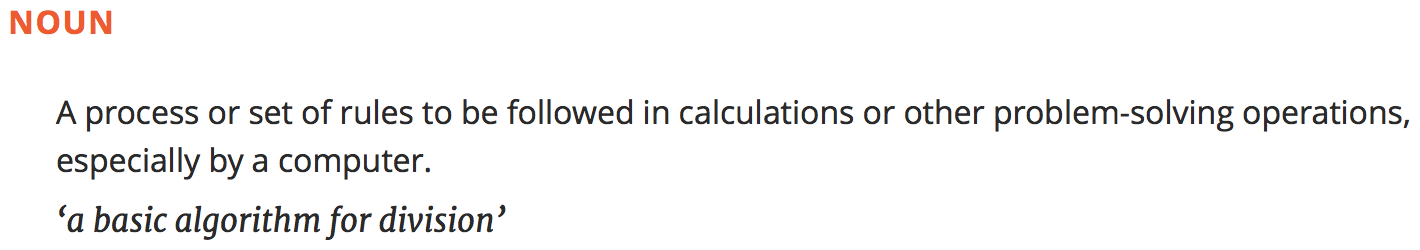
\includegraphics[scale=0.5]{algorithm}
\caption{Algorithm definition taken from the Oxford English Dictionary.}
\label{fig:algorithm}
\end{figure}

As we can see above, it is a "process or set of rules" followed by a computer when trying to solve a problem. As a machine is, at its core, composed of 1s and 0s, a human being needs to visualise what is going under the hood in order to comprehend the steps that are undertaken. In a study conducted by Cristopher D. Hundhausen et al.~\cite{av}, it was proven that even though algorithm visualisation is not the "perfect" solution, it is definitely effective in teaching students and experienced developers.

There are many tools out there that already provide this functionality, but one thing was a key factor in deciding how to proceed with planning the whole software process: there are barely any standalone applications. Even though one can find many websites which let people visualise algorithms' steps (e.g. a great example is VisuAlgo ~\cite{visualgo}), this is not such a good solution as the user cannot use the application at his/her commodity, an Internet connection being required.

Therefore, the plan was to create an app that can be run offline and would feel natural to the user regardless of the operating system of choice. There are many Java implementations (i.e. resulting in jar executables), but one of the main drawbacks is the lack of proper GUI tools that can build native-feeling applications. 

As such, the decision was made to use the Electron framework originally built by the team behind the Atom text editor. This framework uses only web tools to generate executables for all 3 main OS families (i.e. macOS, Windows and Linux) that provide the user with a native, modern and responsive feel. 

The planning was made using the best agile practices~\cite{agile-methodologies}, eventually deciding on following a variation of XP programming. Designing and coming up with an architectural plan was a major milestone to be reached as it took a considerable amount of time to be put in place. However, as it will be discussed in future chapters, the implementation of the animation engine was a crucial and time consuming challenge that required the highest amount of effort.

The report also presents how the app was test in many various ways, as well as how it was evaluated using potential end users. In the end, we shall discuss about the roadmap of the project, why open source is and will be vital for the development of the animator as well as some final thoughts and lessons learned throughout the process.

\section{Aims}

The goals of the project were set and subsequently refined throughout many project meetings, as well as meeting with some fellow classmates to get feedback along the way. 

The main aims of the Algorithm Animator, however, have always been:
\begin{itemize}
	\item Create an efficient and easy-to-use animator.
	\item Make the animator a cross-platform application that would run natively on the main operating system families: macOS, Windows and Linux.
	\item Provide a user-friendly interface that would make the user want to enjoy the product.
	\item Create at least 5-6 fully functional algorithms.
	\item Make the application scalable and easy to maintain.
	\item Test all functionality and ensure quality above quantity.
	\item Evaluate the product throughout the software process to meet acceptance criteria.
	\item Build a roadmap that would allow the animator grow even after the level 4 project has finished.
\end{itemize}

\section{Motivation}

Even if we have previously mentioned that visualising algorithms is one of the best ways of understanding how they perform, there are many other key motivational aspects behind the need of building an animator.

One such 



\section{Contributions}

This report serves to deliver certain main contributions:

\begin{itemize}
	\item Shows the whole software development lifecycle of an algorithm animator.
	\item Presents various technologies used to build native and modern desktop apps~\cite{electron}~\cite{visjs}
	\item Provides a brief overview of current animators available and background knowledge on their benefits and efficiency in teaching.
\end{itemize}


\section{Report Content}
The rest of the report will analyse the background of animators and why they were proven useful, as well as cover all the steps in gathering requirements, designing, implementing, testing and evaluating the tool. 

\begin{itemize}
\item Chapter~\ref{background} covers work related to the purpose of algorithm animators and why they are useful 
\item Chapter~\ref{requirements} goes into how the problem was analysed and what requirements were gathered through
	project meetings and discussions with Algorithmics students.
\item Chapter~\ref{planning} shows the steps undertaken to follow the best agile methodology principles.
\item Chapter~\ref{design} explains the design decisions behind the tool and illustrates various lessons learned and
	problems faced along the way.
\item Chapter~\ref{implementation} goes into the implementation details of the animator.
\item Chapter~\ref{testing} show how extensive unit, integration and other types of testing (e.g. smoke, end-to-end)
	were undergone and why they were essential to the development of the application.
\item Chapter~\ref{conclusions} details the overall results of the project.
\end{itemize}

%==============================================================================

\chapter{Background}
\label{background}

\section{Related Work}

%==============================================================================

\chapter{Requirements}
\label{requirements}

\section{Problem Analysis}

\section{Requirements Gathering}

\section{Functional Requirements}

\section{Non-Functional Requirements}

%==============================================================================

\chapter{Planning}
\label{planning}

\section{Agile}

\subsection{Kanban Board}

\subsection{Issues \& Bug Tracking}

%==============================================================================

\chapter{Design}
\label{design}

\section{Architecture}

\subsection{EDA (Event-driven Architecture)}

\section{Native Desktop App vs. Jar}

\section{Electron}

\section{Vis.js}

\section{Material Design}

\section{Compromises}

%==============================================================================

\chapter{Implementation}
\label{implementation}

\section{Project Structure}

\section{JavaScript and Multi-Threading}

\section{JS Animation Engine}

\section{Extra Features}

\section{Lessons Learned}

\section{Issues Faced}

%==============================================================================

\chapter{Testing}
\label{testing}

\section{Unit Testing}

\section{Integration Testing}

\section{Prototype Evaluation}

\section{Results}

%==============================================================================

\chapter{Conclusions}
\label{conclusions}

\section{Open Source}

\section{Project Roadmap}

\section{Final Thoughts}

\section{Acknowledgements}

\bibliographystyle{plain}
\bibliography{l4proj}
\end{document}
